\documentclass[letterpaper]{article}
\usepackage{proceed2e}
\usepackage{times}
\usepackage{helvet}
\usepackage{courier}
\usepackage{epsfig,subfigure}
\usepackage{amsmath,amsfonts,amssymb,amsthm}
\usepackage{array}
% Import some more mathematical symbols
\usepackage{amsmath,amssymb}

% Import an algorithm formatting package
\usepackage[vlined,algoruled,titlenumbered,noend]{algorithm2e}

% Define argmin, argmax
\def\argmax{\operatornamewithlimits{arg\max}}
\def\argmin{\operatornamewithlimits{arg\min}}
\def\supmax{\operatornamewithlimits{arg\sup}}

% Strikeout
%\usepackage{ulem}
%\normalem

% Define a fourth level subheading (Scott)
\newcommand{\subfour}{\vspace*{3mm}\hspace{-2mm}}
\renewcommand{\-}{\text{-}}

% Define a command for extended commenting (Scott)
\long\def\COMMENT#1\ENDCOMMENT{\message{(Commented text...)}\par}

% Define common macros
\long\def\COMMENT#1\ENDCOMMENT{\message{(Commented text...)}\par}

\newtheorem{lemma}{Lemma}[section]
\newtheorem{assumption}[lemma]{Assumption}
\newtheorem{theorem}[lemma]{Theorem}
\newtheorem{proposition}[lemma]{Proposition}
\newtheorem{corollary}[lemma]{Corollary}
\newtheorem{hypothesis}[lemma]{Hypothesis}
\newtheorem{definition}[lemma]{Definition}
%\newtheorem{hypothesis}{Hypothesis}{\bfseries}{\itshape}
%\theoremstyle{remark}
%\newtheorem*{proof_deferred}{Proof}
%\newtheorem*{proofsk}{Proof Sketch}{\rmfamily}{\rmfamily}

% No brackets after {definition},{example} starts new counters 
\newtheorem{property}[lemma]{Property}
\newtheorem{example}[lemma]{Example}

\newcommand{\norm}[1]{\textrm{\normalsize $#1$}}
\newcommand{\sm}[1]{\textrm{\footnotesize $#1$}}

\newcommand{\denselist}{\itemsep 0pt\partopsep 0pt}
\newcommand{\semidenselist}{\itemsep 2pt\partopsep 2pt}

%\def\casemax{\operatornamewithlimits{case\,max}}
\def\argmax{\operatornamewithlimits{arg\,max}}
\def\argmin{\operatornamewithlimits{arg\,min}}

%\def\argmax{\mathop{\rm arg\,max}}

%\numberwithin{algorithm}{chapter}

\newcommand{\casemax}{\textrm{casemax}}
\newcommand{\B}{\mathbb{R}}
\newcommand{\R}{\mathbb{R}}
\newcommand{\I}{\mathbb{I}}
\newcommand{\E}{\mathbb{E}}
\newcommand{\F}{\mathcal{F}}
\newcommand{\G}{\mathcal{G}}
\newcommand{\X}{\mathcal{X}}
\newcommand{\op}{\;\mathit{op}\;}

\newcommand{\D}{\mathcal{D}}
\newcommand{\II}{\mathcal{I}}
\newcommand{\Gain}{\mathit{Gain}}
\newcommand{\VPI}{\mathit{VPI}}

\newcommand{\var}{v}
\newcommand{\eq}{\leftarrow}

\newcommand{\LB}{\mathit{LB}}
\newcommand{\UB}{\mathit{UB}}

\renewcommand{\vec}[1]{\mathbf{#1}}

\renewcommand{\l}{\langle}
\renewcommand{\r}{\rangle}

% Macro for strikeout text
\newlength{\howlong}
\newcommand{\sout}[1]{
\settowidth{\howlong}{#1}%
#1\unitlength0.5ex%
\begin{picture}(0,0)
\put(0,1){\line(-1,0){\howlong\divide\unitlength}}
\end{picture}%
}





\begin{document}
% The file aaai.sty is the style file for AAAI Press 
% proceedings, working notes, and technical reports.
%
% exact symbolic bayesian inference for piecewise priors and likelihoods
\title{Symbolic Methods for Exact Gibbs Sampling in Piecewise Bayesian Models}

% WinBUGS Manual
%
%d) Logical nodes cannot be given data or initial values. This means,
%   for example, that it is not possible to model observed data that 
%   is the sum of two random variables. (See Logical nodes.)
%
% See further notes on truncation and censoring... more restrictions
% but need to understand better.  Indeed we likely give an automated 
% method for working out the algebra for truncated distributions as
% they suggest.

\author{Anonymous}
%\author{Ehsan Abbasnejad\\
%ANU \& NICTA\\
%Canberra, Australia\\
%{\tt ehsan.abbasnejad@nicta.com.au}
%\And
%Scott Sanner\\
%NICTA \& ANU\\
%Canberra, Australia\\
%{\tt scott.sanner@nicta.com.au}
%}

\maketitle

\begin{abstract}
In Bayesian probabilistic models, it is often useful to have piecewise
priors or likelihoods, e.g., a uniform distribution with latent upper
bounds constrained to be greater than latent lower bounds, or an
observation that is the maximum of latent random variables.
Unfortunately, standard inference toolkits such as Bayesian inference
using Gibbs sampling (BUGS) are unable to derive samplers for these
two examples, leading researchers to use alternative approximate
inference techniques without asymptotic guarantees, or to simply avoid
such piecewise models altogether.  In this work, we show how to
compute closed-form integrals on piecewise functions with
deterministic variable dependencies (via symbolic collapsing) and
furthermore, to exploit recently developed data structures for
efficiency of these operations.  Empirically, this enables us to
perform exact Gibbs sampling in the previous two examples while also
scaling to accommodate large piecewise Bayesian graphical models such
as those required for pairwise preference learning or learning from
range-restricted score data.  As a result, this work enables
sampling-based Bayesian inference in a novel range of piecewise models
for which automated Gibbs samplers were previously unknown.
%- Exact inference known, but as we will show, not scalable.
%- First exact Gibbs sampler for arbitrary linear piecewise polynomial likelihoods ().
%- New methods for working with delta functions with logical distributions.
%- Piecewise likelihoods are pervasive in *many* important Bayesian inference problems
%  hard boundaries, truncation at 0, max functions, etc.
%  (people currently approximate heavily)
\end{abstract}

% \cite{}, \citeauthor{}~\shortcite{} (to include author names in text)

\section{Introduction}

\label{sec:intro}

There are many cases in Bayesian modeling where it is useful (and
sometimes, required) to have priors or likelihoods that are piecewise;
we examine two such cases in Figure~\ref{gm:uniform_max}.  In
\ref{gm:uniform_max}(a), we have observed data in the maximum range
$[0,m]$ ($m > 0$) generated from a uniform distribution with latent
upper bound $u$ and lower bound $l$ where the joint prior on $l$ and
$u$ must enforce $u > l$; we would like to obtain a posterior over $u$
and $l$ in this model.  In \ref{gm:uniform_max}(b), we have observed
maximum bid data from a number of sealed bid auctions where the
bidders are known, but only the winning bid value is revealed; then we
would like to obtain a posterior over each bidder's unknown valuation
$b_i$ of the given commidity.  Later in our empirical results section
we will further discuss cases of preference learning and inference
from restricted range score data where piecewise likelihoods and
priors are appropriate.

Despite the wide range of settings in which such piecewise Bayesian
models could be useful, there are few options for inference in such
models with strong guarantees:
%in these models that guarantee asymptotic convergence to the exact value
\begin{itemize}
\item Closed-form approximation techniques such as variational message
  passing~\cite{} or expectation propagation~\cite{} have proved
  effective for many specific Bayesian inference
  tasks~\cite{lda,trueskill,matchbox}, but lack asymptotic exactness
  guarantees.
\item Exact closed-form inference techniques based on symbolic
  variable elimination (SVE)~\cite{sve} have been proposed for factor
  graphs with piecewise factors, but have two caveats: (1) in
  practice, SVE inference is superexponential in the number of
  variables in the model, and (2) SVE cannot currently handle the
  $\delta$ function in Figure~\ref{gm:uniform_max}.  Nonetheless, SVE
  does provide a foundation for exact symbolic inference that we build
  on in this work.
% MH not effective for high-dimensional models as used in experiments?
% - Or do an MH step in a Gibbs step?  
% - Or do a slice sampling in a Gibbs step?  But need to know all regions
% with value >= to the slice, which is difficult and requires zero-finding
% when multimodal.
\item Markov Chain Monite Carlo (MCMC)~\cite{hastings70,mcmc} sampling
  methods such as Metropolis-Hastings (MH)~\cite{} or Gibbs
  sampling~\cite{geman} \emph{do} have asymptotic exactness
  guarantees.  While MH is often used in practice, it requires a
  proposal distribution and step size that should be properly tuned to avoid slow
  convergence, especially in the case of multimodal
  posteriors~\cite{}, which are exacerbated in the case of piecewise
  models as we show later.
\end{itemize}
% TODO: should show this later or remove!
On the other hand, Gibbs sampling~\cite{geman} does not require
tuning in practice but does require the automatic derivation of
conditional probabilities for each latent variable in the Bayesian
probabilistic model.  The well-known Bayesian inference using
Gibbs Sampling (BUGS) software~\cite{winbugs} in fact performs
this automatic derivation for conjugate priors and uses a variety
of other specialized techniques including MH, slice sampling~\cite{neal}
for non-conjugate cases.  However, ***
for a large subset of piecewise models with latent bound parameters
as in Figure~\ref{gm:uniform_max}(a) or evidence that is a deterministic
function of two or more latent variables as required to encode
the inference problem of Figure~\ref{gm:uniform_max}(b).

% Derive the direct conditional!  No MH steps, etc.
To obtain a completely automatic inference approach for piecewise
Bayesian models with asymptotic exactness guarantees and 
no tuning of a proposal distribution required, we focus on Gibbs sampling
in this work and 

% Winbugs does not allow logical functions or children to take data,
% except for certain link functions so in following, x cannot take
% data:
% - x = a + b
% - x = a * b
% - x = max(a, b)
% - x = step(a>b, 0)
% Logical nodes are used to transform observed data and to make
% derived functions whose value is sampled.  Nodes downstream of
% a logical node of a stochastic variable only seem to be generated
% in a feedforward process, they never feed back.
%
% *** While BUGS cannot handle x = a + b, if a and b are Gaussian
%     then tons of methods can handle this problem so delta substitution
%     is rather obvious here.  Delta substitution really only interesting
%     with piecewise functions like max.
%
% It does not support joint / piecewise priors, say I[a>b] on uniform,
% does allow step(a+b > 0), but the output is a variable.
%
% It cannot handle truncated distributions with unknown bounds since
% the normalizing constant is dependent on the bounds.  To handle this,
% we would need symbolic integration with parameters in denominator.
%
% It seems logical variables should not have stochastic children, only
% stochastic parents?
%
% Does conditional distribution work out?  How to work with delta function?
% Does it induce determinism?  For max model?  For score model?
Hard!

Two contributions:


In many interesting Bayesian graphical models, the prior or likelihood
may be piecewise functions.  For e

, e.g., a uniform distribution with unknown
upper bound constrained to be greater than the lower bound, or an
observation that is the maximium of latent random variables.
Unfortunately, standard toolkits such as Bayesian inference using
Gibbs sampling (BUGS) are unable to derive samplers for such models,
leading researchers to use alternative approximate inference
techniques without guarantees on convergence, or to simply avoid these
piecewise models altogether.  In this work, we show how to compute
closed-form integrals on piecewise functions with deterministic
variable dependencies and furthermore, to exploit recently developed
data structures for efficiency of these operations. 

%that render exact inference computationally intractable.  
%While recent work has developed a linear piecewise
%polynomial model that is a conjugate prior for an expressive family of
%piecewise prior and likelihood distributions with the caveat that the
%complexity of inference is super-exponential in the size of the model,
%making it intractable for practical inference.  
In this work, we make two major contributions over and above this
previous work: (1) we show how logical nodes often used in Bayesian
graphical models can be used in conjunction with previous work, and
(2) we show how exact Gibbs samplers can be derived for any graphical
model over piecewise polynomial factors and linear piecewise logical
nodes (notably including piecewise functions such as maximization).
This work marks the first time that an exact Gibbs sampling method can
be fully automated for this expressive class of piecewise Bayesian
models (e.g., inference not possible in BUGS), making possible
automated inference in a range of novel models such as A, B, and C
that we empirically evaluate and show D, E, and F.

%%%%%%%%%%%%%%%%%%%%%%%%%%%%%%%%%%%%%%%%%%%%%%%%%%%%%%%%%%%%%%%%%%%%%%%%%%
%\begin{minipage}{\textwidth}
\begin{figure}[t!]
\centering
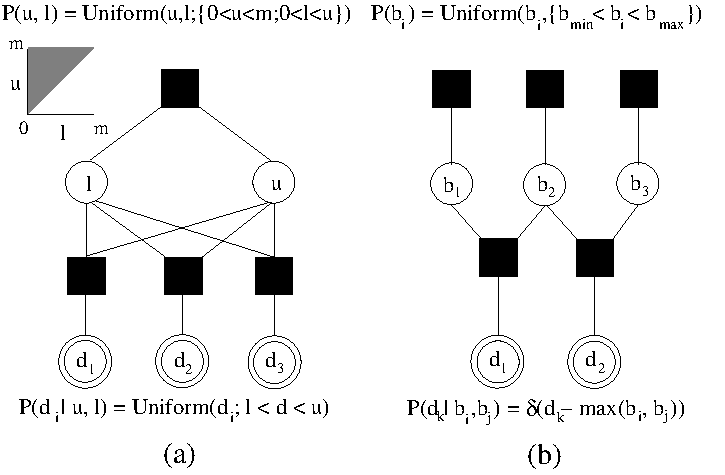
\includegraphics[width=.50\textwidth]{uniform_max.pdf}
\vspace{-6mm}
\caption{\footnotesize Two piecewise Bayesian models: 
(a) data samples $d_i$ are generated uniformly from a uniform with 
upper bound $u$ and lower bound $l$ having a joint uniform prior where $u > l$;
(b) data samples $d_k$ are observations of the maximum bid $b_i$ and $b_j$
in a sealed bid auction with a uniform prior over the range of each bid.}
\label{fig:uniform_max}
%\caption{\footnotesize .} 
\vspace{-4mm}
\end{figure}
%\end{minipage}
%%%%%%%%%%%%%%%%%%%%%%%%%%%%%%%%%%%%%%%%%%%%%%%%%%%%%%%%%%%%%%%%%%%%%%%%%%


% TODO:
%
% Explain why distributions are useful (example)
% - Convex polytopes
% - Explain logical nodes and things like max, or uniform with unknown
% - Show model and an example posterior
% Explain why result in AAAI 2012 is surprising (oblique polynomials)
% - Cannot be handled by BUGS, slice sampling
% - Different from other methods: Infer.net, Church (Metropolis Hastings)
%   suffers from inefficiency of proposal
% Key is closed-form automated integration operations on linear piecewise 
%   polynomial functions and linear piecewise delta functions -- operations for
%   which integration was not previously known to be closed-form


% Max function
% Dynamics
% Expectations of arbitrary functions if allowing delta function!

Real-world probabilistic reasoning is rife with uncertainty over
continuous random variables with complex (often nonlinear)
relationships, e.g., estimating the position and pose of entities from
measurements in robotics, or radar tracking applications with
asymmetric stochastic dynamics and complex mixtures of noise
processes.  While closed-form exact solutions exist for inference in
some continuous variable graphical models, such solutions are largely
limited to relatively well-behaved cases such as joint Gaussian
models.  On the other hand, the more complex inference tasks of
tracking with real-world sensors involves underlying distributions
that are beyond the reach of current closed-form exact solutions.
Take, for example, the robot sensor model in Figure~\ref{fig:gm2}
motivated by~\cite{thrun_mcl}.

Here $d \in \R$ is a variable representing the distance of a
mobile robot to a wall and $x_i$ are the observed measurements of
distance (e.g., using a laser range finder).  The prior distribution
$P(d)$ is uniform $U(d;0,10)$ while the observation model
$P(x_i|d)$ is a \emph{mixture} of three distribitions: (red) is a
truncated Gaussian 
representing noisy measurements $x_i$ of the actual
distance $d$ within the sensor range of $[0,10]$; 
(green) is a uniform noise model $U(d;0,10)$
representing random anomalies leading to any measurement; and
(blue) is a triangular distribution peaking at the maximum measurement
distance (e.g., caused by spurious deflections of laser light or the 
transparency of glass).

While our focus in this paper is on exact inference in \emph{general}
discrete and continuous variable graphical models and not purely on
this robotics localization task, this example clearly motivates the
real-world need for reasoning with complex distributions over
continuous variables.  However, in contrast to previous work that has
typically resorted to (sequential) Monte Carlo
methods~\cite{thrun_mcl,particle_filters} to perform inference in this
model (and dynamic extensions) via 
\emph{sampling}, our point of departure in this work is to seek \emph{exact,
closed-form solutions} to general probabilistic inference tasks in
these graphical models, e.g., arbitrary conditional probability 
queries or conditional expectation computations.

To achieve this task, we focus on an expressive class of mixed
discrete and continuous variable Bayesian networks whose conditional
probability functions can be expressed as piecewise polynomials with
bounded support (where piece boundaries must be inequalities of linear
functions).  In practice, this representation is sufficient to
represent or arbitrarily approximate a wide range of common
distributions such as the following: uniform (piecewise constant),
triangular (piecewise linear), truncated normal
distributions\footnote{In practice, measurements have natural ranges
that make truncated variants of distributions appropriate, e.g., a
range finder that exhibits Gaussian distributed measurement errors but
only returns measurements in the range $[0,10]$ may be well-suited to
a truncated Normal distribution observation model.}  (piecewise
quadratic or quartic), as well as all mixtures of such distributions
as exemplified in $P(x_i|d)$ above (since a sum of piecewise
polynomials is still piecewise polynomial).  While polynomials
directly support the integrals we will need to compute \emph{variable
elimination}~\cite{varelim} in closed-form, computing the definite
integrals of polynomials w.r.t.\ arbitrary linear piece boundaries
turns out to be a much more difficult task achieved through novel
\emph{symbolic} methods that underlie the key contribution of
\emph{symbolic variable elimination (SVE)} that we make in this paper.

% E[d|x_1] example?
In the following sections, we present our graphical model
framework using a \emph{case} representation of probability
distributions followed by a description of our SVE procedure.  
After this, we introduce
the \emph{extended algebraic decision diagram (XADD)} --- a practical
data structure for efficiently and compactly manipulating the case
representation --- and apply XADD-based SVE to robotics localization 
and a tracking tasks demonstrating exact closed-form inference 
for these problems.  

\section{Discrete and Continuous Graphical Models}

\subsection{Factor Graph Representation}

A discrete and continuous \emph{graphical model} compactly represents
a joint probability distribution $p(\vec{b},\vec{x})$ over an
assignment $(\vec{b},\vec{x}) = ( b_1,\ldots,b_n,x_{1},\ldots,x_m )$
to respective random variables $(\vec{B},\vec{X}) =
(B_1,\ldots,B_n,X_{1},\ldots,X_m )$.\footnote{Notational comments:
we sometimes abuse notation and treat
vectors of random variables or assignments as a set, e.g., 
$(\vec{b},\vec{x}) = \{ b_1,\ldots,b_n,x_1,\ldots,x_m \}$.  
Also we often do
not distinguish between a random variable (upper case) and its
realization (lower case), e.g., $p(x_1) := p(X_1 = x_1)$.}  Each $b_i$
($1 \leq i \leq n$) is boolean s.t.\ $b_i \in \{ 0,1 \}$ and each
$x_j$ ($1 \leq j \leq m$) is continuous s.t.\ $x_j \in \R$.

As a general representation of both directed and undirected graphical
models, we use a \emph{factor graph}~\cite{factor_graph} 
representing a joint probability $p(\vec{b},\vec{x})$ as a
product of a finite set of factors $F$, i.e.,
\vspace{-2mm}
{\footnotesize
\begin{equation}
p(\vec{b},\vec{x}) = \frac{1}{Z} \prod_{f \in F} \Psi_f(\vec{b}_f,\vec{x}_f).
\label{eq:fg}
\vspace{-1mm}
\end{equation}
}
Here, $\vec{b}_f$ and $\vec{x}_f$ denote the subset of variables that
participate in factor $f$ and $\Psi_f(\vec{b}_f,\vec{x}_f)$ is a 
non-negative, real-valued 
potential function that can be viewed as gauging the local
compatibility of assignments $\vec{b}_f$ and $\vec{x}_f$.  
The functions $\Psi_f$ may not necessarily represent probabilities and
hence a normalization constant $Z$ is often required to ensure
$\sum_{\vec{b}} \int_{\vec{x}} p(\vec{b},\vec{x}) d\vec{x} = 1$.

We will specify all of our algorithms on graphical models in terms of 
general factor graphs, but we note that \emph{Bayesian networks} represent
an important modeling formalism that we will use to specify our examples
in this paper.  For the Bayesian network directed graph 
in the introductory example, the joint distribution
for $n$ variables is represented as the product of all variables
conditioned on their parent variables in the graph and can be
easily converted to factor graph form, i.e., 
{{\footnotesize
\vspace{-2mm}
\begin{align}
p(d,x_1,\ldots,x_k) \; & = \; p(d) \prod_{i=1}^k p(x_i|d) \nonumber \\
& = \; \psi_d(d) \prod_{i=1}^k \Psi_{x_i} (x_i,d) \label{eq:bn}
\vspace{-1mm}
\end{align}
}
where quite simply, $\Psi_{d} (d) := p(d)$ and $\Psi_{x_i} (x_i,d) :=
p(x_i|d)$.  Here, $Z=1$ and is hence omitted since joint distribitions
represented by Bayesian networks marginalize to 1 by definition.

%These definitions hold for general (conditional) probability density
%functions and their corresponding factors; subsequently 
%we will specify a restricted factor representation for 
%piecewise polynomial functions, which can be conveniently represented
%in a mathematical case notation.

\subsection{Variable Elimination Inference}

Given a joint probability distribution $p(\vec{b},\vec{x})$
defined by a factor graph, our objective in this paper will
be to perform two types of \emph{exact, closed-form} inference:

%\begin{itemize}
%\item 
{\bf (Conditional) Probability Queries:} for query
$\vec{q}$ and disjoint (possibly empty) 
evidence $\vec{e}$ drawn from 
a subset of $(\vec{b},\vec{x})$, we wish to infer 
the \emph{exact}
form of $p(\vec{q}|\vec{e})$ as a \emph{function} of 
$\vec{q}$ and $\vec{e}$.  This can be 
achieved by the following computation, where 
for notational convenience we assume variables are renamed s.t. 
$\{ \vec{b} \cup \vec{x} \} \setminus \{ \vec{q} \cup \vec{e} \} = ( b_1,\ldots,b_s,x_1,\ldots,x_t)$ and 
$\vec{q} = (b_{s+1},\ldots,b_{s'},x_{t+1},\ldots,x_{t'})$:
{\footnotesize
\begin{align}
& p(\vec{q}|\vec{e}) = \label{eq:cprob}\\
& = \frac{\sum_{b_1} \cdots \sum_{b_s} \int \cdots \int_{\mathbb{R}^t} \prod_{f \in F} \Psi_f(\vec{b}_f,\vec{x}_f) \, dx_1 \ldots dx_t}
{\sum_{b_1} \cdots \sum_{b_{s'}} \int \cdots \int_{\mathbb{R}^{t'}} \prod_{f \in F} \Psi_f(\vec{b}_f,\vec{x}_f) \, dx_1 \ldots dx_{t'}} \nonumber
\end{align}
}
The $\frac{1}{Z}$ from~\eqref{eq:fg} would appear in \emph{both}
the numerator and denominator and hence cancels.

%\item
{\bf (Conditional) Expectation Queries:} for a continuous
query random variable
$Q$ and disjoint evidence assignment $\vec{e}$ drawn from 
a subset of $(\vec{b},\vec{x})$, we wish to infer 
the \emph{exact value} of $\E[Q|\vec{e}]$.\footnote{We do not 
discuss the expectation of $\{0,1\}$ boolean
random variables $B$ since $\E[B|\vec{e}] = P(B=1|e)$, which can 
already be computed in~\eqref{eq:cprob}.} 
This can be achieved by the following
computation, where $p(q|\vec{e})$ can be pre-computed according to~\eqref{eq:cprob}:
%$\vec{q} = \{ b_{s'+1},\ldots,b_{s''},x_{t'+1},\ldots,x_{t''} \}$:
\vspace{-0.5mm}
{\footnotesize 
\begin{equation} 
\E[Q|\vec{e}] = 
%\sum_{b_{s'+1}} \cdots \sum_{b_{s''}} 
%\int_{x_{t'+1}=-\infty}^{\infty} \cdots \int_{x_{t''}=-\infty}^{\infty} 
\int_{q=-\infty}^{\infty} [q \cdot p(q|\vec{e})] \, dq \label{eq:cexp}
\vspace{-0.5mm}
\end{equation}
}
%Here, $p(q|\vec{e})$ is computed using the conditional probability 
%query expression in~\eqref{eq:cprob}.
%\end{itemize}

\emph{Variable elimination (VE)}~\cite{varelim} is a simple and
efficient algorithm given in Algorithm~\ref{alg:varelim} that exploits
the distributive law to \emph{efficiently} compute each elimination
step (i.e., any $\sum_{b_{i}}$ or $\int_{x_{j}}$ in~\eqref{eq:cprob}
and~\eqref{eq:cexp}) by first factorizing out all factors independent
of the elimination variable; this prevents unnecessary multiplication
of factors, hence minimizing the size and complexity of each
elimination operation.  If the factor representation is closed and
computable under the VE operations of multiplication and
marginalization then VE can compute any (conditional) probability or
expectation query in~\eqref{eq:cprob} and~\eqref{eq:cexp}.  
Closed-form, exact solutions for VE are well-known for the discrete
and joint Gaussian cases; next we extend VE to expressive
piecewise polynomial discrete/continuous graphical models.

%Providing a factor representation for
%continuous graphical models that is closed under 
%all VE operations (other than the joint Gaussian case) 
%is the problem we address next.

%%%%%%%%%%%%%%%%%%%%%%%%%%%%%%%%%%%%%%%%%%%%%%%%%%%%%%%%%%%%%%%%%
\incmargin{1.5em}
\linesnumbered
\begin{algorithm}[hb!]
\SetKwFunction{eliminate}{{\sc Eliminate}}
\SetKwInOut{Input}{input}
\SetKwInOut{Output}{output}
\dontprintsemicolon

\Input{$F,\mathit{order}$: a set of factors $F$, and a variable 
$\mathit{order}$ for elimination}
\Output{a set of factors after eliminating each $\var \in \mathit{order}$}
\BlankLine
{\small
\Begin{
   \emph{// eliminate each $\var$ in the given $\mathit{order}$}\\
   \ForEach{$\var \in \mathit{order}$}{
     \emph{// multiply $\otimes$ all factors containing $\var$}\\ 
     \emph{// into $f_\var$, put other factors in $F_{\setminus \var}$}\\
     $f_\var \eq 1$; $F_{\setminus \var} \eq \emptyset$\;
     \ForEach{$f \in F$}{
       \lIf{($f$ contains $\var$)\;}{
	 $f_\var \eq f_\var \otimes f$\;
       }\lElse{
	 $F_{\setminus \var} \eq F_{\setminus \var} \cup \{ f \}$\;
       }
     }
     %$\qquad$\\%\vspace{3mm}
     \emph{// eliminate var; insert result into factor}\\
     \emph{// set $F$ along with $F_{\setminus \var}$}\\
     \lIf{($\mathit{var}$ is boolean)\;}{
       $F \eq F_{\setminus \var} \cup \{ \sum_{\var \in \{0,1\}} f_\var \}$\;
     }\lElse{
       $F \eq F_{\setminus \var} \cup \{ \int_{\var=-\infty}^{\infty} f_\var \, d\var \}$
     }
   }
   \Return{$F$}\;
}
}
\caption{{\sc VE}($F,\mathit{order}$)  \label{alg:varelim}}
\end{algorithm}
\decmargin{1.5em}
%%%%%%%%%%%%%%%%%%%%%%%%%%%%%%%%%%%%%%%%%%%%%%%%%%%%%%%%%%%%%%%%%

\section{Symbolic Variable Elimination in Discrete/Continuous Graphical Models}

As discussed previously, piecewise polynomial functions provide an
expressive framework for representing discrete/continuous variable
graphical models when all distributions have bounded support.  In this
section, we introduce a case notation and operations for piecewise
polynomials, define factor graphs in terms of these case statements,
and show that all VE operations, including definite
integration w.r.t.\ multivariate piecewise polynomial functions, can
be computed in exact, closed-form using a purely \emph{symbolic}
representation, hence the algorithm \emph{Symbolic VE} (SVE).

\subsection{Case Representation and Operators}

For this section, we will assume all functions
are represented in \emph{case} form as follows:
\vspace{-1mm}
{%\footnotesize 
\begin{align}
f = 
\begin{cases}
  \phi_1 & f_1 \\ 
  \vdots & \vdots \\ 
  \phi_k & f_k \\ 
  \vspace{-6mm}
\end{cases} \label{eq:case}
\end{align}
} 
Here, the $f_i$ may be polynomials of $\vec{x}$ with non-negative
exponents.  The $\phi_i$ are logical formulae defined over
$(\vec{b},\vec{x})$ that can consist of arbitrary conjunctions of (a)
(negated) boolean variables in $\vec{v}$ and (b) inequalities
($\geq,>,\leq,<$), equalities ($=$), or disequalities ($\neq$) where
the left and right operands must be \emph{linear} functions.  We
assume that the set of conditions $\{ \phi_1,\ldots,\phi_k \}$ 
disjointly and exhaustively partition $(\vec{b},\vec{x})$ such that $f$
is well defined for all $(\vec{b},\vec{x})$.  It is easy to verify
that such a representation can represent the uniform and triangular
distributions and arbitrarily approximate the truncated normal 
distribution required to specify $p(x_i|d)$ discussed in 
the introduction.

% TODO: Examples

\emph{Unary operations} such as scalar multiplication $c\cdot f$ (for
some constant $c \in \mathbb{R}$) or negation $-f$ on case statements
$f$ are straightforward; the unary operation is simply applied to each
$f_i$ ($1 \leq i \leq k$). Intuitively, to perform a \emph{binary
  operation} on two case statements, we simply take the cross-product
of the logical partitions of each case statement and perform the
corresponding operation on the resulting paired partitions.  Thus, we 
perform the ``cross-sum'' $\oplus$ of two (unnamed) cases as follows:
\vspace{-1mm}
{\footnotesize 
\begin{center}
\begin{tabular}{r c c c l}
&
\hspace{-6mm} 
  $\begin{cases}
    \phi_1: & f_1 \\ 
    \phi_2: & f_2 \\ 
  \end{cases}$
$\oplus$
&
\hspace{-4mm}
  $\begin{cases}
    \psi_1: & g_1 \\ 
    \psi_2: & g_2 \\ 
  \end{cases}$
&
\hspace{-2mm} 
$ = $
&
\hspace{-2mm}
  $\begin{cases}
  \phi_1 \wedge \psi_1: & f_1 + g_1 \\ 
  \phi_1 \wedge \psi_2: & f_1 + g_2 \\ 
  \phi_2 \wedge \psi_1: & f_2 + g_1 \\ 
  \phi_2 \wedge \psi_2: & f_2 + g_2 \\ 
  \end{cases}$
\end{tabular}
\end{center}
}
\normalsize
Likewise, we perform $\ominus$ and $\otimes$ by,
respectively, subtracting or multiplying partition values (rather than
adding them) to obtain the result.  
%If the operands are well-defined functions then it is easy to see
%the result will be as well.
Some partitions resulting from
the application of the $\oplus$, $\ominus$, and $\otimes$ operators
may be inconsistent (infeasible); if we can detect this (e.g., via
a linear constraint solver), we may simply discard such 
partitions as they are irrelevant to the function value.

For variable elimination, we'll need to compute definite integrals
 --- a fairly non-trivial operation
that is discussed in its own section.  But first we discuss 
maximization (needed for working with integral bounds) and restriction
(needed to compute marginals for boolean variables).

\emph{Symbolic maximization} is fairly straightforward
to define if we note that the conditional nature of the
case statements allows us to directly encode maximization:
\vspace{-1mm}
{\footnotesize
\begin{center}
\begin{tabular}{r c c c l}
&
\hspace{-9mm} $\max \Bigg(
  \begin{cases}
    \phi_1: & f_1 \\ 
    \phi_2: & f_2 \\ 
  \end{cases}$
\hspace{-1mm}
$,$
&
\hspace{-5mm}
  $\begin{cases}
    \psi_1: & g_1 \\ 
    \psi_2: & g_2 \\ 
  \end{cases} \Bigg)$
&
\hspace{-5mm} 
$ = $
&
\hspace{-5mm}
  $\begin{cases}
  \phi_1 \wedge \psi_1 \wedge f_1 > g_1    : & f_1 \\ 
  \phi_1 \wedge \psi_1 \wedge f_1 \leq g_1 : & g_1 \\ 
  \phi_1 \wedge \psi_2 \wedge f_1 > g_2    : & f_1 \\ 
  \phi_1 \wedge \psi_2 \wedge f_1 \leq g_2 : & g_2 \\ 
  \phi_2 \wedge \psi_1 \wedge f_2 > g_1    : & f_2 \\ 
  \phi_2 \wedge \psi_1 \wedge f_2 \leq g_1 : & g_1 \\ 
  \phi_2 \wedge \psi_2 \wedge f_2 > g_2    : & f_2 \\ 
  \phi_2 \wedge \psi_2 \wedge f_2 \leq g_2 : & g_2 \\ 
  \end{cases}$
\end{tabular}
\end{center}
}
The key observation here is that case statements are closed under the
max operation.  While it may appear that this representation will lead
to an unreasonable blowup in size, we note the XADD that we introduce
later will be able to exploit the internal decision structure of this
maximization to represent it much more compactly.

% TODO: Edit here... boolean only
The two operations required for marginalization over boolean variables
$b$ are $\oplus$ and \emph{restriction} of variable $b$ in factor $f$
to the value $x \in {0,1}$, written as $f|_b=x$.
For $x = 1$ ($x = 0$), $f|_b=x$ simply requires instantiating all
variables $b$ in $f$ with $x$.  For example, let
\vspace{-1mm}
\begin{align*}
f = \begin{cases}
    \phi_1 \land b: & f_1 \\ 
    \phi_2 \land \neg b: & f_2 \\ 
    \phi_3 : & f_3 \\ 
  \end{cases}
  \vspace{-3mm}
\end{align*}
then the two possible restrictions of $b$ yield the following 
results (where inconsistent case partitions have been removed):
\vspace{-4mm}
\begin{align*}
f|_{b=1} = \begin{cases}
    \phi_1: & f_1 \\ 
    \phi_3: & f_3 \\ 
  \end{cases}
\hspace{10mm}
f|_{b=0} = \begin{cases}
    \phi_2: & f_2 \\ 
    \phi_3: & f_3 \\ 
  \end{cases}.
  \vspace{-4mm}
\end{align*}

\subsection{Definite Integration of the Case Representation}

\label{sec:def_int}

One of the major technical contributions of this paper is the symbolic
computation of the definite integration required to eliminate
continuous variables in SVE.  If we are 
computing $\int_{x_1=-\infty}^{\infty} f \, dx_1$ for $f$ 
in~\eqref{eq:case}, we can rewrite it in the following equivalent form
\vspace{-2mm}
{\footnotesize
\begin{equation}
\int_{x_1=-\infty}^{\infty} \sum_i \I[\phi_i] \cdot f_i \, dx_1 \; = \; \sum_i \int_{x_1=-\infty}^{\infty} \I[\phi_i] \cdot f_i \, dx_1 \label{eq:int_decomp}
\vspace{-1mm}
\end{equation}
}
where $\I[\cdot]$ is an indicator function taking value 1 when
its argument is true, 0 when it is false.  Hence we can compute
the integrals separately for each case partition (producing a 
case statement) and then $\sum$ the results using $\oplus$.

To continue with the integral for a single case partition, we
introduce a concrete example.  Let $f_1 := x_1^2 - x_1 x_2$ and $\phi_1
:= [x_1 > -1] \land [x_1 > x_2-1] \land [x_1 \leq x_2] \land [x_1 \leq x_3 +1] \land [x_2 > 0]$.  
In computing $\int_{x_1=-\infty}^{\infty} \I[\phi_1] \cdot f_1 \, dx_1$,
the first thing we note is that the constraints involving $x_1$ in
$\I[\phi_1]$ can be used to restrict the integration range for $x_1$.
In fact, we know that the integrand is only non-zero for
$\max(x_2 - 1, -1) < x_1 \leq \min(x_2,x_3 + 1)$.  Using the $\max$
operation defined previously, we can 
write explicit functions in 
\emph{piecewise polynomial case form} for the respective 
lower and upper bounds $\LB$ and $\UB$:
{\footnotesize
\vspace{-1mm}
\begin{align*}
\LB &:=\begin{cases}
    x_2-1 > -1:&\hspace{-2mm} x_2 - 1 \\ 
    x_2-1 \leq -1:&\hspace{-2mm} -1 \\ 
  \end{cases}\;
\UB &:=\begin{cases}
    x_2<x_3+1:&\hspace{-2mm} x_2 \\ 
    x_2\geq x_3+1:&\hspace{-2mm} x_3 + 1 \\ 
  \end{cases}
\end{align*}
}
Now we can rewrite the integral as\footnote{The careful reader will note
that because the lower bounds were defined in terms of $>$
rather than $\leq$, we technically have an improper integral
and need to take a limit.  However, in taking the limit, we
note that all integrands are continuous polynomials
of order 0 or greater, so the limit exists and yields the
same answer as substituting the limit value.  Hence for 
polynomials, we need not be concerned about whether bounds
are inclusive or not.}
\vspace{-1mm}
\begin{equation}
\I[x_2 > 0] \int_{x_1=\LB}^{\UB} (x_1^2 - x_1 x_2) \, dx_1 .
\end{equation}
Note here that $\I[x_2 > 0]$ is independent of $x_1$ and hence
can factor outside the integral.  With all indicator functions
moved into the $\LB$ or $\UB$ or factored out, we can now compute
the integral:
\vspace{-1mm}
{\footnotesize
\begin{equation}
\I[x_2 > 0] \left[ \frac{1}{3}x_1^3 - \frac{1}{2}x_1^2 x_2 \bigg|_{x_1=\LB}^{x_1=\UB} \right] .
\end{equation} }
The question now is simply how to do this evaluation?  Here we note
that every expression (variables, constants, indicator functions, etc.) 
can be written as a 
simple case statements or as operations on case statements, even the upper
and lower bounds as shown previously.  So the evaluation is simply 
\vspace{-1mm}
{\footnotesize
\begin{align}
\I[x_2 > 0] \otimes \bigg[ & \left( \frac{1}{3} \UB \otimes \UB \otimes \UB \ominus \frac{1}{2} \UB \otimes \UB \otimes (x_2) \right) \nonumber \\
& \hspace{-8mm} \ominus \left( \frac{1}{3} \LB \otimes \LB \otimes \LB \ominus \frac{1}{2} \LB \otimes \LB \otimes (x_2) \right) \bigg] \label{eq:almost_final}.
\end{align}
}
Hence the result of the definite integration over a case
partition of a piecewise polynomial function with linear constraints
is simply a case statement in the same form --- 
this is somewhat remarkable given that
all of the bound computations were symbolic.  Furthermore, one might
fear that high-order operations like $\UB \otimes \UB \otimes \UB$
could lead to a case partition explosion, but we note this example simply
has the effect of cubing the expressions in each partition of $\UB$ since
all case partitions are disjoint.

However, we are not yet done, there is one final step that we must
include for correctness.  Because our bounds are symbolic, it may be
the case for some assignment to $(\vec{b},\vec{x})$ that $\LB \geq
\UB$.  In this case the integral should be zero since the constaints
on $x_1$ could not be jointly satisfied.  To enforce this
symbolically, we simply need to $\otimes$~\eqref{eq:almost_final} by
case statements representing the following inequalities for all pairs
of upper and lower bounds:
{\footnotesize
\begin{equation}
\I[x_2 > x_2 - 1] \otimes \I[x_2 > -1] \otimes \I[x_3 + 1 > x_2 - 1] \otimes \I[x_3 + 1 > -1]
\end{equation}}
Of course, here $\I[x_2 + 1 > x_2 - 1]$ could be removed as a tautology,
but the other constraints must remain.

This provides the solution for a single case partition and 
from~\eqref{eq:int_decomp}, we just need to $\oplus$ the case
statements from each case partition integral evaluation to obtain
the full integral, \emph{still in piecewise polynomial case form}.

%So to recap, isolate variable on LHS of constraint, 
%LB is max of RHS of $>$, $\geq$ constraints,
%UB is min of RHS $<$, $\leq$ constraints,
%write in case form.
%then take max LB, min UB

% Write out case as sum, focus on an individual partition

% Remove constraints independent of integration var, put in CONS

% Analyze all constraints on integration var, divide into UB and LB

% Use min(LB) and max(UB), add in indicator constraint to CONS

% Substitute (see Ehsan's bars)... requires recursively recomputing
% the result from a case statement viewing every constraint
% as a product of indicator functions, and every expression as
% case operations on leaf nodes, substituting the case statement
% in for the var as needed... result is a case statement!
%
% Note: efficient for polynomial operations since disjoint!

% Multiply by CONS and keep running sum... XADD introduced later
% will ensure that the result is maintained compactly.

\subsection{Piecewise Polynomial Factor Graphs and Symbolic Variable Elimination (SVE)}

We define a factor graph from~\eqref{eq:fg} with factors represented
by our case formalism as \emph{piecewise polynomial factor graphs
(PPFGs)}.  
%\begin{restr}[Case Factor Restriction for PPFGs]
%Given
%variable elimination $\mathit{order}$, for all PPFG factors
%$f(\vec{v})$, the $v \in \vec{v}$ occurring earliest in
%$\mathit{order}$ may only occur linearly in any of the constraints
%$\phi_i$ of factor $f(\vec{v})$.
%\end{restr}
%\vspace{-1mm}
With the preceding machinery, generalizing VE to Symbolic VE (SVE) for
PPFGs is straightforward.  We need only replace all sums and products
in VE with the case versions $\oplus$ and $\otimes$.  Then the only
operation we need to specify in the VE Algorithm~\ref{alg:varelim} is
to define the computation for the variable
eliminations.  For PPFGs, there are two cases:

\vspace{2mm}
{\bf Discrete Variable Elimination} (line 14 of VE):\\
\vspace{-3mm}
$$\sum_v f_v := f_v|_{v=1} \oplus f_v|_{v=1}.$$
\vspace{-2mm}
{\bf Continuous Variable Elimination} (line 15 of VE):\\ 
$$\int_{\var=-\infty}^{\infty} f_\var \, d\var := \mbox{(see definite integration)}$$.

Each elimination operation takes operands in the previously defined
case form and produces operands in this same form --- crucially this means
that the piece constraints always remain linear.  Importantly for the
complex operation of definite integration, this means that the upper
and lower bounds can always be isolated in order to evaluate the
integral.  Since definite integration and all other
required SVE operations preserve the case property, 
all SVE operations can be computed on an PPFG in closed-form.

This completes the definition of SVE.  If the exact model could be
represented as a PPFG, then SVE provides exact closed-form inference.
Otherwise one can approximate most graphical models to arbitrary
precision using PPFGs --- once this is done, SVE will provide exact
inference in this approximated model.

%%%%%%%%%%%%%%%%%%%%%%%%%%%%%%%%%%%%%%%%%%%%%%%%%%%%%%%%%%%%%%%%%%%%%%%%%%
%\begin{figure*}[t!]
%\begin{center}
%\vspace{-1mm}
%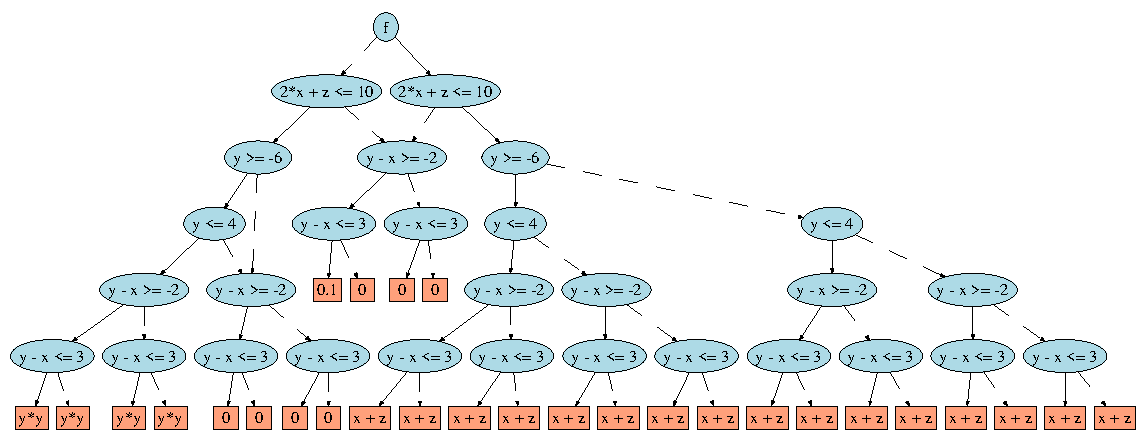
\includegraphics[width=1.0\textwidth]{norm_unif_tree.pdf}
%\end{center}
%\vspace{-2mm}
%\caption{\footnotesize A tree representation of a case statement; each branch corresponds to a single case partition.} \label{fig:xadd_tree}
%%\vspace{-2mm}
%\end{figure*}
%%%%%%%%%%%%%%%%%%%%%%%%%%%%%%%%%%%%%%%%%%%%%%%%%%%%%%%%%%%%%%%%%%%%%%%%%%

\section{Extended ADDs (XADDs) for Case Statements}

In practice, it can be prohibitively expensive to maintain a case
statement representation of a value function with explicit partitions.
Motivated by algebraic decision diagrams (ADDs)~\cite{bahar93add},
which maintain compact representations for finite discrete functions,
we use an extended ADD (XADD) formalism introduced 
in~\cite{uai11} and demonstrated in 
Figure~\ref{fig:xadd}.\footnote{Our usage of the XADD differs
from~\cite{uai11} in that it was used there to represent
\emph{deterministic equations} over continuous variables, whereas
here we use it to represent polynomial condition \emph{probability
densities}.  \cite{uai11} did not discuss \emph{definite integration} in XADDs,
but the adaptation of this operation 
from case statements to XADDs is straightforward.}

%%%%%%%%%%%%%%%%%%%%%%%%%%%%%%%%%%%%%%%%%%%%%%%%%%%%%%%%%%%%%%%%%%%%%%%%%%
\begin{figure}[t!]
\begin{center}
\vspace{-1mm}
\fbox{Placeholder}%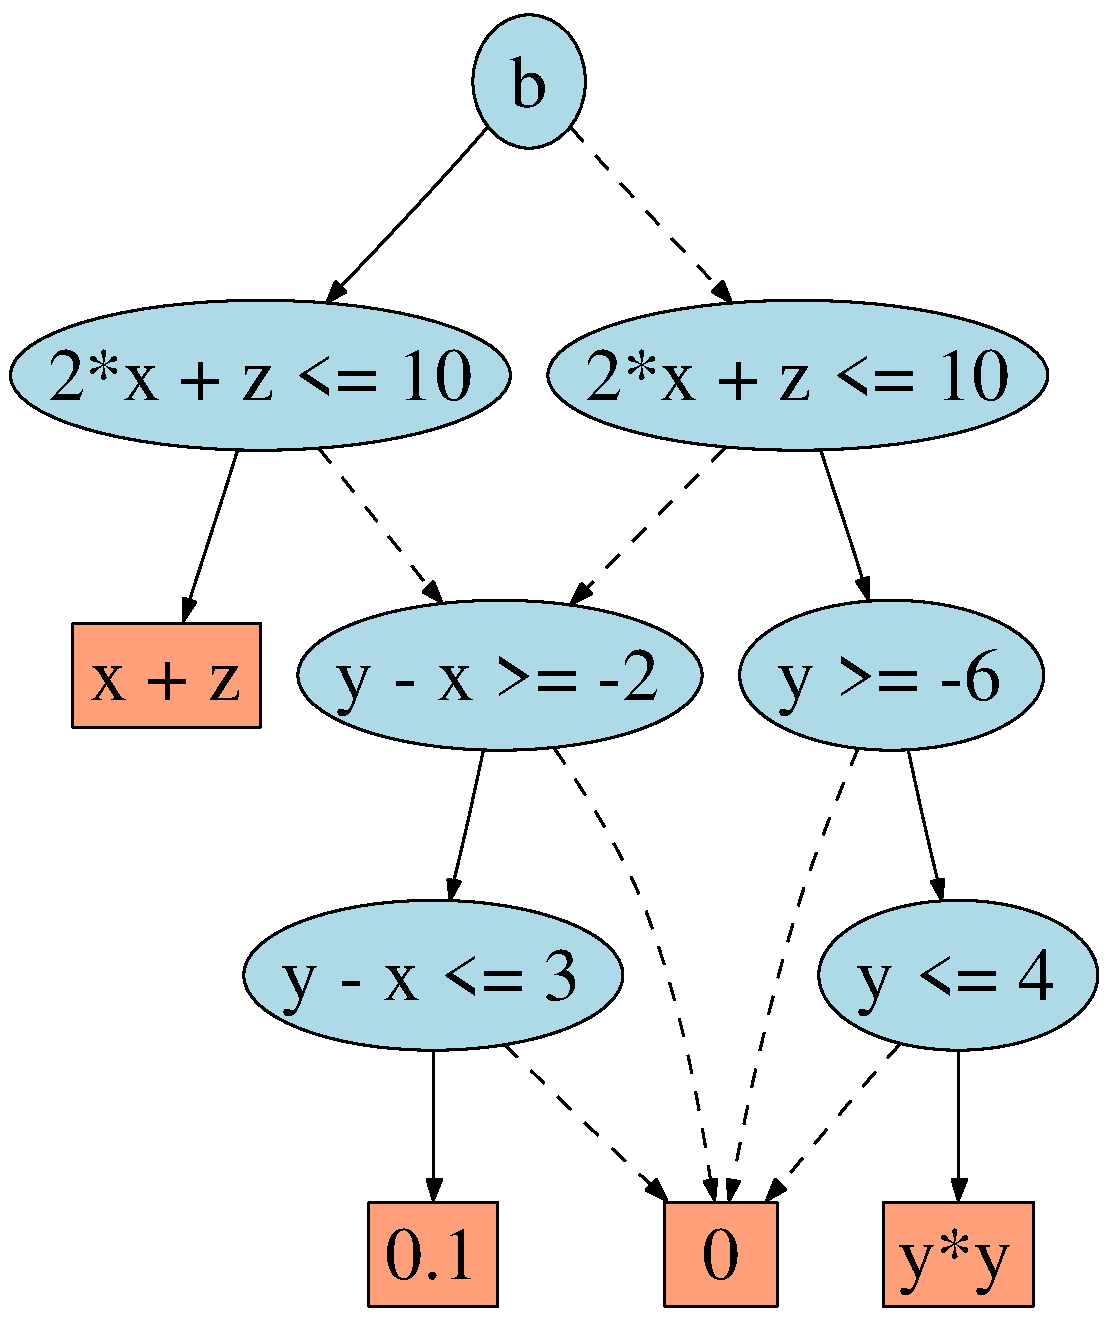
\includegraphics[width=.2\textwidth]{norm_unif.pdf}
\end{center}
\vspace{-2mm}
\caption{\footnotesize An XADD example from a case statement.% in Figure~\ref{fig:xadd_tree}.
} \label{fig:xadd}
\vspace{-4mm}
\end{figure}
%%%%%%%%%%%%%%%%%%%%%%%%%%%%%%%%%%%%%%%%%%%%%%%%%%%%%%%%%%%%%%%%%%%%%%%%%%

The XADD is like an algebraic decision 
diagram (ADD)~\cite{bahar93add} except that (a) the decision
nodes can have arbitrary inequalities or (dis)equalities (one
per node) and (b) the leaf nodes can represent arbitrary functions.
The decision nodes still have a fixed order from root to leaf
and the standard ADD
operations to build a canonical ADD (\textsc{Reduce}) and 
to perform a binary operation on two ADDs (\textsc{Apply}) 
still applies in the case of XADDs. 

Of particular importance is that the XADD is a directed acyclic graph
(DAG), and hence is often much more compact than a tree
representation, e.g., as demonstrated in 
Figure~\ref{fig:xadd}.
%in Figure~\ref{fig:xadd_tree} we provide the function represented by the XADD in Figure~\ref{fig:xadd} expanded from a DAG into it's tree form.  
We remark that not only are XADDs compact on account of their
reconvergent DAG structure (each path from root to leaf would be a separate
case partition), but that all unary and binary operations
on XADDs can directly exploit this compact structure for efficiency.

It is fairly straightforward for XADDs to support all case operations
required for SVE.  Standard operations like unary multiplication,
negation, $\oplus$, and $\otimes$ are implemented exactly as they
are for ADDs.  For the maximization operation, when two leaf
nodes $f$ and $g$ are reached and they are general expressions,
the additional decision node $f > g$ is introduced to represent
the maximum.  This may occasionally introduce out-of-order decisions
which can be easily detected and repaired as discussed in~\cite{uai11} .

\section{Empirical Results}

\section{Concluding Remarks}

\bibliography{baypw}
\bibliographystyle{plain}

\end{document} 
